\section{Architekturen}

\plain{MY-NEUPOWER}

\subsection{MY-NEUPOWER}
\begin{slide}{MY-NEUPOWER}
	\begin{itemize}
		\item von Hitachi Microcomputer System Ltd. (1998)
		\item SIMD parallel Computer
		\item Neuronen als eigene Processing-Elements
		\item Broadcast-Bus zwischen allen PEs
		\item SCSI interface
		\item 25 MHz
		\item 512 physische Neuronen
		\item bis zu 4096 logische Neuronen
	\end{itemize}
\end{slide}

\begin{slide}{MY-NEUPOWER}
	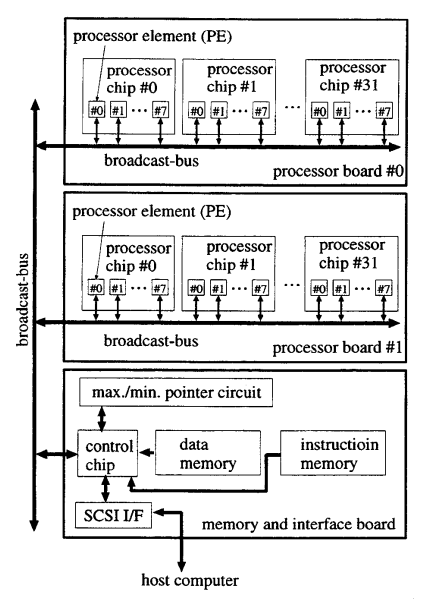
\includegraphics[width=\textwidth,height=0.8\textheight,keepaspectratio]{content/neupower2}
	\blfootnote{Yasunaga, Moritoshi, Akio Yamada, and Tatsuo Okahashi. "Performance of a bus-based parallel computer with integer-representation processors applied to artificial neural network and parallel AI domains." IEEE, 1998.}
\end{slide}

\begin{slide}{MY-NEUPOWER}
	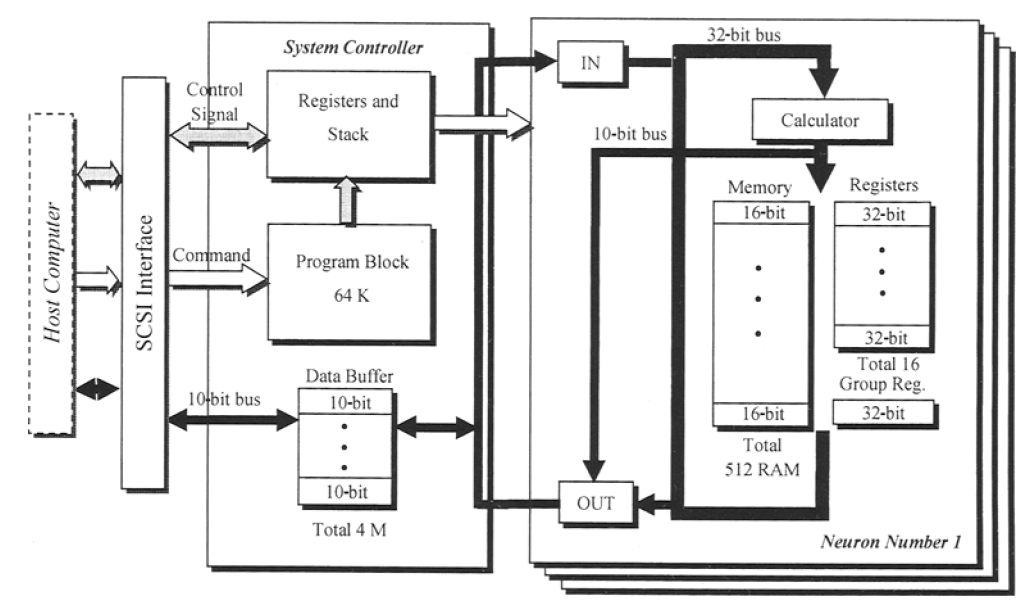
\includegraphics[width=\textwidth,height=0.8\textheight,keepaspectratio]{content/neupower}
	\blfootnote{Sugisaka, Masanori, and Zhi-Jun Liu. "The application of a neurocomputer for a control problem." Artificial Life and Robotics 3.4, 1999.}
\end{slide}

